\documentclass[10pt]{amsart}
% \usepackage[showboxes]{textpos}

\usepackage[absolute,overlay]{textpos}
	\setlength{\TPHorizModule}{1.0cm}
	\setlength{\TPVertModule}{\TPHorizModule}
	\textblockorigin{0.0cm}{0.0cm}  %start all at upper left corner
 
\usepackage{amsmath}
\usepackage{amsthm}
\usepackage{amsfonts}
\usepackage{amssymb} 
\usepackage{mathpazo}
\usepackage{booktabs}
\usepackage[usenames,x11names]{xcolor}
\usepackage{tikz}
\usepackage{textcomp}
\usepackage[letterpaper]{geometry}
\geometry{verbose,tmargin=0.5in,bmargin=0.5in,lmargin=0.75in,rmargin=0.5in}
\usepackage{multicol}
\usepackage{bm}
\usepackage{comment}
\usepackage{cancel}
\usepackage{array}
\usepackage{gensymb}
\usepackage{enumerate}   

\pagestyle{plain}
\raggedright 
\renewcommand{\familydefault}{\sfdefault}
\setlength{\parskip}{\medskipamount}
\setlength{\columnsep}{1cm}
 
\everymath{\displaystyle}
\setlength{\parskip}{\bigskipamount}

\input{../../macros}

\begin{document} 

\thispagestyle{empty}
\vspace{-7cm}
\centering


\textbf{\Large Module 5: Friction Losses (CIVL 318)}
\par\medskip
\begin{center}
	\begin{tabular}{r >{$}r<{$} >{$}c<{$} >{$}l<{$}}
		\toprule
		\addlinespace
		\textbf{ Reynolds Number}: & N_R &=& \frac{vD\rho}{\eta}  \\
		\addlinespace
		& N_R < 2000 & \Rightarrow & \text{laminar} \\
		\addlinespace
		& 2000 < N_R < 4000 & \Rightarrow & \text{critical flow} \\
		
		\addlinespace
		& N_R > 4000 & \Rightarrow & \text{turbulent flow} \\
		\addlinespace
		\midrule
		\addlinespace	
		\textbf{Laminar flow:} & f &=& \frac{64}{N_R} \\
		\addlinespace
		\midrule
		\addlinespace
		\textbf{Turbulent flow:}: & f &=&
		\frac{0.25}{\left[\log\left(\frac{1}{3.7\left(D/\epsilon\right)}+\frac{5.74}{N_R^{0.9}}\right)\right]^2}  \\
		\addlinespace	
		\midrule
		\addlinespace
		\textbf{ Darcy's Equation}: & h_L &=& f\times \frac{L}{D}\times\frac{v^2}{2g}  \\
		\addlinespace			
		\bottomrule				
	\end{tabular}
	
	\vspace{2cm}
	
	
	\textbf{Roughness, $\epsilon$}:
	\par\bigskip
	\begin{tabular}{rrl}
		\toprule
		Material (new, clean) & $\qquad$ & $\epsilon$ (m)\\
		\midrule
		\midrule
		Glass & & Smooth\\
		\midrule
		Plastic &  & $3.0\times10^{-7}$\\
		\midrule
		Copper, brass, lead (tubing) &  & $1.5\times10^{-6}$\\
		\midrule
		Commercial steel, welded steel &  & $4.6\times10^{-5}$\\
		\midrule
		Wrought iron &  & $4.6\times10^{-5}$\\
		\midrule
		Ductile Iron - coated &  & $1.2\times10^{-4}$\\
		\midrule
		Ductile Iron - uncoated &  & $2.4\times10^{-4}$\\
		\midrule
		Concrete &  & $1.2\times10^{-4}$\\
		\midrule
		Riveted steel &  & $1.8\times10^{-3}$\\
		\midrule
		\bottomrule
	\end{tabular}
	\par
	
	
\end{center}

%%%%%%%%%%%%%%%%%%%%%%%%%%%%%%%%%%%%%%%%%%%%%%%%%%%%%%%%%%%%%%%%%%%%%%%%%%%%%%%%%%%%%%%%%%%%%%%%%%%%%%%%%%%%%%%%%%%%%

% \rule{\textwidth}{0.02in}
%%%%%%%%%%%%%%%%%%%%%%%%%%%%%%%%%%%%%%%%%%%%%%%%%%%%%%%%%%%%%%%%%%%%%%%%%%%%%%%%%%%%%%%%%%%%%%%%%%%%%%%%%%%%%%%%%%%%%
\newpage

\begin{multicols}{2}
\raggedright 

%%%%%%%%%%%%%%%%%%%%%%%%%%%%%%%%%%%%%%%%%%%%%%%%%%%%%%%%%%%%%%%%%%%%%%%%%%%%%%%%%%%%%%%%%%%%%%%%%%%%%%%%%


	\textbf{Example 1}:
		Flow is said to be in the \textbf{critical region}, with neither fully laminar or fully turbulent flow, if the Reynolds number for the 
		flow is between $2000$ and $4000$.
		\par\medskip
		Determine the range of velocities and volume flow rates for which flow is in the critical region for:
		\par\medskip
		\begin{enumerate}
		  \item water at $5$\textcelsius{} flowing in $1/2$-in copper tubing 
		  \item water at $95$\textcelsius{} flowing in $1/2$-in copper tubing
		  \item fuel oil at $10$\textcelsius{} ($\text{sg}=0.94$, $\eta=2.4\;\mathsf{Pa\cdot s}$), \newline flowing in $12$-in Schedule $40$ steel pipe
		\end{enumerate}
	
% 	\textbf{Solution}:\\
% 	(1)
% 	From tables in the text or provided, $\rho=1000\;\mathsf{kg/m^3}$, $ \eta=1.52\times 10^{-3}\;\mathsf{Pa\cdot s}$ and
% 	$D=13.39\text{ mm}$ so:
%   	\begin{align*}  		
%   		2000 &= \frac{v_{2000}(0.01339)(1000)}{1.52\times10^{-3}}\\
%   		v_{2000} &= 0.22704\text{ m/s}\\
%   		4000 &= \frac{v_{4000}(0.01339)(1000)}{1.52\times10^{-3}}\\
%   		v_{4000} &= 0.45407\text{ m/s}\\\\
%   		Q_{2000} &= \pi(0.01339\text{ m})^2/4\times 0.22704\text{ m/s}\\
%   			&= 3.1971\times10^{-5}\mathsf{m^3/s}\\
%   			&= 0.031971\text{ L/s}\\
%   			Q_{4000} &= 0.063942\text{ L/s}
%   	\end{align*}
%   	For flow to remain in the critical region:
%   	\begin{align*}
%   		0.22704\text{ m/s} < &v < 0.45407\text{ m/s}\\
%   		0.031971\text{ L/s} < &Q < 0.063942\text{ L/s}
%   	\end{align*}
%  
%   
% 	(2)
% 	$\rho=962\;\mathsf{kg/m^3}$ and $ \eta=2.92\times 10^{-4}\;\mathsf{Pa\cdot s}$ so:
%   	\begin{align*}
%   		N_R &= \frac{vD\rho}{\eta}\\
%   		2000 &= \frac{v_{2000}(0.01339)(962)}{2.92\times10^{-4}}\\
%   		v_{2000} &= 0.045337\text{ m/s}\\
%   		v_{4000} &= 0.090675\text{ m/s}\\\\
%   		Q_{2000} &= \pi(0.01339\text{ m})^2/4\times 0.045337\text{ m/s}\\
%   			&= 6.3842\times10^{-6}\mathsf{m^3/s}\\
%   			&= 0.0063842\text{ L/s}\\
%   			Q_{4000} &= 0.012765\text{ L/s}\\
%   	\end{align*}
%   	
%   	For most situations, water flow is fully turbulent.
%   	\par\bigskip
%   	
%   	(3)
%   	$\rho=940\;\mathsf{kg/m^3}$, $ \eta=2.4\;\mathsf{Pa\cdot s}$ and $D=303.2\text{ mm}$ so:
%   	\begin{align*}
%   		2000 &= \frac{v_{2000}(0.3032)(962)}{2.4}\\
%   		v_{2000} &= 16.842\text{ m/s}\\
%   		v_{4000} &= 33.683\text{ m/s}\\\\
%   		Q_{2000} &= \pi(0.3032\text{ m})^2/4\times 16.842\text{ m/s}\\
%   			&= 7.5715\times10^{-6}\mathsf{m^3/s}\\
%   			&= 1.2160\;\mathsf{m^3/s}\\
%   			Q_{4000} &= 2.4320\;\mathsf{m^3/s}
%   	\end{align*}
%   	\par\vspace{\stretch{1}}
% 	
% \columnbreak
\vfill
\pagebreak
%%%%%%%%%%%%%%%%%%%%%%%%%%%%%%%%%%%%%%%%%%%%%%%%%%%%%%%%%%%%%%%%%%%%%%%%%%%%%%%%%%%%%%%%%%%%%%%%%%%%%%%%%%%%%%%%%%%%%
\Large	


	\textbf{Example 2}:
	
		Determine the headloss due to friction in fuel oil at $10$\textcelsius{} flowing through $125\text{ m}$ 
			of $12$-in Schedule $40$ steel pipe with an average flow velocity of $4.5\text{ m/s}$. \par\medskip
			Then determine the headloss if the average flow velocity is reduced to $2.25\text{ m/s}$.\par\medskip 
			($\text{sg}=0.94$, $\eta=2.4\;\mathsf{Pa\cdot s}$).\par\medskip


% 	\textbf{Solution}:
% 	First, we must calculate the Reynolds number:
% 	\begin{align*}
% 		N_R &= \frac{vD\rho}{\eta}\\
% 		&=\frac{4.5\times 0.3032\times 940}{2.4}\\
% 		&= 534.39
% 	\end{align*}
% 	Flow is laminar ($N_R<2000$) so $f=\frac{64}{N_R}=0.11976$\par
% 	Use Darcy's Equation to calculate the head loss:
% 	\begin{align*}
% 		h_L &= f\times \frac{L}{D}\times\frac{v^2}{2g}\\
% 		&=0.11976\times\frac{125}{0.3032}\times\frac{4.5^2}{2g}\\
% 		&= 50.960\text{ m}
% 	\end{align*}
% 	Now, calculate the headloss at $2.9\text{ m/s}$
% 	\begin{align*}
% 		N_R &= \frac{2.9\times 0.3032\times 940}{2.4}\\
% 		&= 344.38\\\\
% 		f &= \frac{64}{344.38}=0.18584\\\\
% 		h_L	&=0.18584\times\frac{125}{0.3032}\times\frac{2.9^2}{2g}\\
% 		&= 32.841\text{ m}
% 	\end{align*}
% 	Note that, for laminar flow, $h_L\propto v$
% 	\par\medskip Note also that a loss of $32.841\text{ m}$ of head is equivalent to an energy loss of $32.841\;\mathsf{N\cdot m}$ of
% 	energy per N of oil. 
% 	
% 	\par\vspace{\stretch{1}}
% 	\pagebreak

\vfill\newpage
	
	\end{multicols}
	
	%%%%%%%%%%%%%%%%%%%%%%%%%%%%%%%%%%%%%%%%%%%%%%%%%%%%%%%%%%%%%%%%%%%%%%%%%%%%%%%%%%%%%%%%%%%%%%%%%%%%%%%%%%%%%%%%%%%%%
	\raggedright
	\textbf{Example 3}	
	Use the Moody diagram to determine the friction factor for flow with $N_R=2\times 10^6$ and a relative roughness of
	1428.\par\bigskip
	\begin{center}
		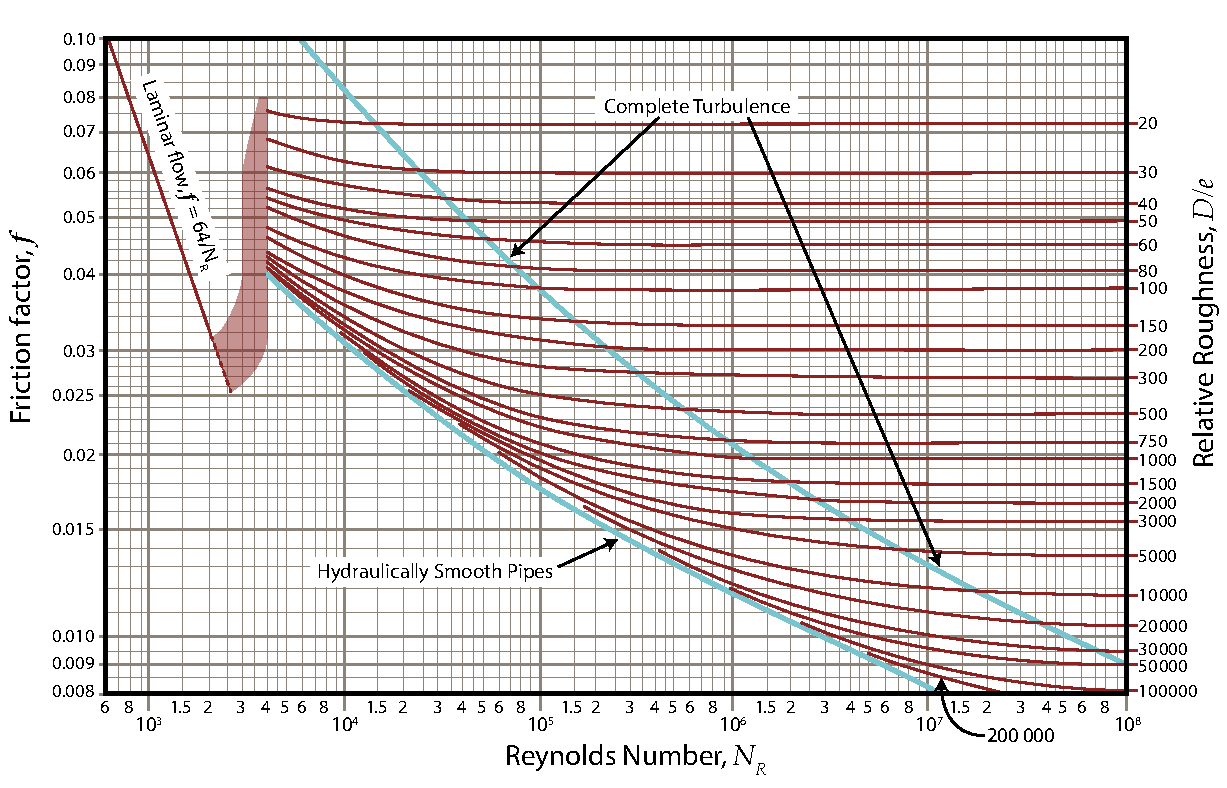
\includegraphics[scale=1.1, angle=90]{../../figs/05FrictionLosses/moody.pdf}
	\end{center}
	
	
	\newpage
	
	%%%%%%%%%%%%%%%%%%%%%%%%%%%%%%%%%%%%%%%%%%%%%%%%%%%%%%%%%%%%%%%%%%%%%%%%%%%%%%%%%%%%%%%%%%%%%%%%%%%%%%%%%%%%%%%%%%%%%
	
	\textbf{Example 4}	
	Use the Moody diagram to determine the friction factor for flow with $N_R=1.6\times 10^5$ and in new clean
	$1/2$-in copper tubing.\par\medskip
	
	\begin{center}
		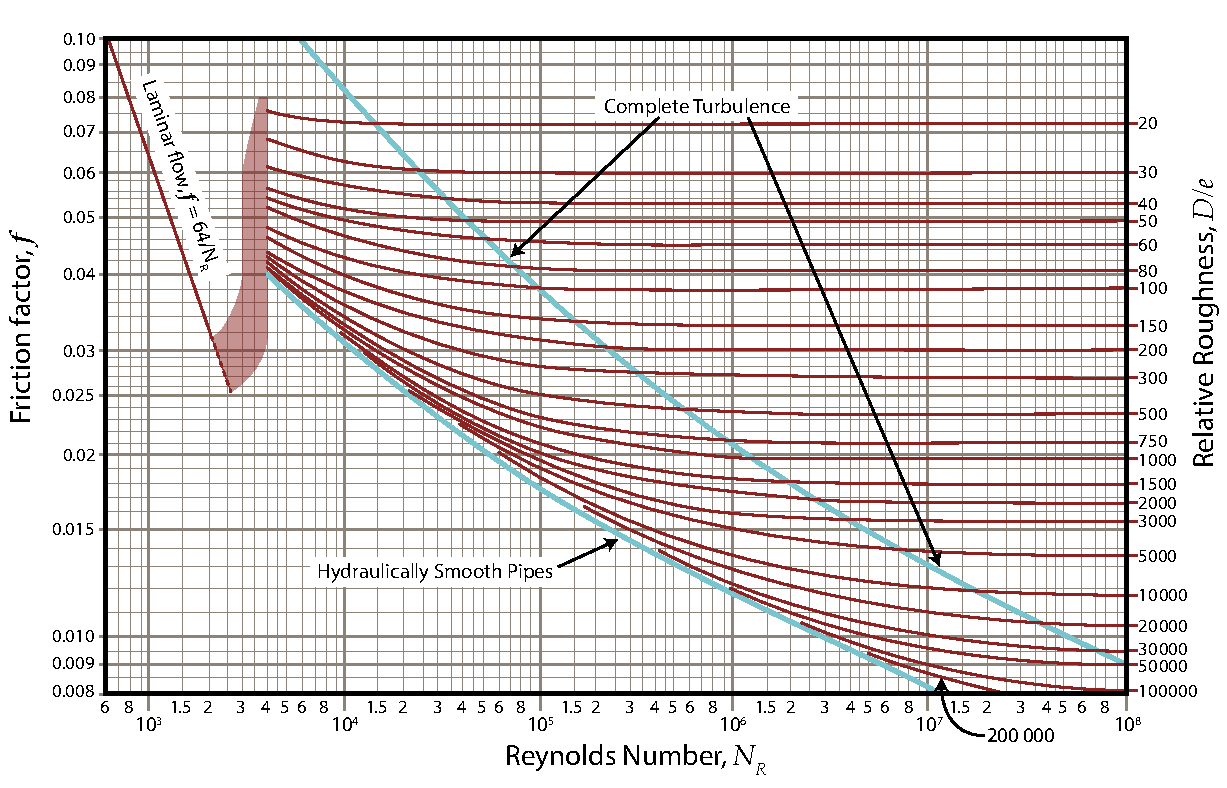
\includegraphics[scale=1.1, angle=90]{../../figs/05FrictionLosses/moody.pdf}
	\end{center}
	
	
	\newpage
	
	%%%%%%%%%%%%%%%%%%%%%%%%%%%%%%%%%%%%%%%%%%%%%%%%%%%%%%%%%%%%%%%%%%%%%%%%%%%%%%%%%%%%%%%%%%%%%%%%%%%%%%%%%%%%%%%%%%%%%
	
	\textbf{Example 5}
	A 75 m section of wooden flume is replaced with 54-in high
density polyethylene (HDPE) pipe with inside diameter of
1.37 m. The pipe is smooth and transports $ 190 \times 10^3\mathsf{\, m3/day}$.
Determine the headloss due to friction in the pipe, assuming
an average temperature of 10 \textcelsius.\par\medskip
	
	\begin{center}
		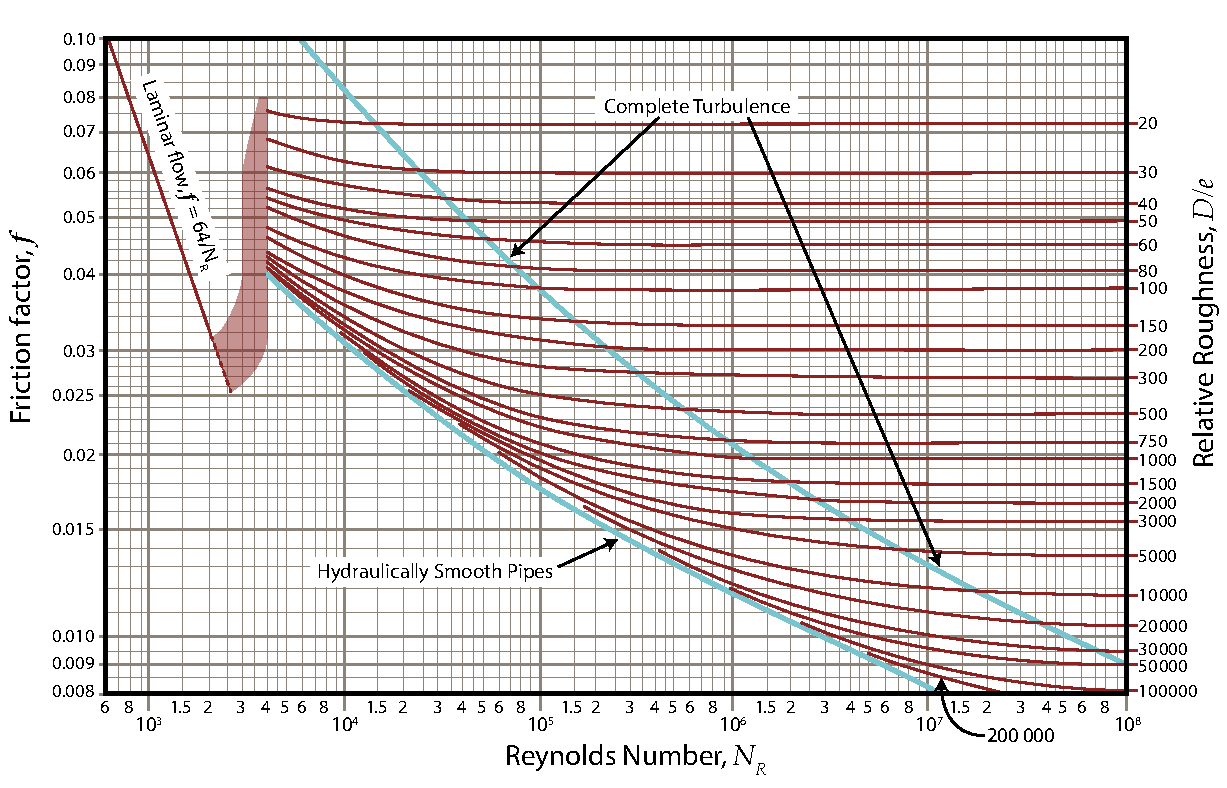
\includegraphics[scale=1.1, angle=90]{../../figs/05FrictionLosses/moody.pdf}
	\end{center}
	
	
	\newpage

%%%%%%%%%%%%%%%%%%%%%%%%%%%%%%%%%%%%%%%%%%%%%%%%%%%%%%%%%%%%%%%%%%%%%%%%%%%%%%%%%%%%%%%%%%%%%%%%%%%%%%%%%%%%%%%%%%%%%
	\begin{multicols}{2}
	
	\textbf{Example 6}:
	
	Ethyl alcohol at $25$\textcelsius{} flows through $1\tfrac{1}{2}\text{-in}$ Schedule $80$ steel pipe at
	$5\text{ L/s}$. Determine the pressure drop, due to friction losses, in a $125\text{ m}$ section of pipe.

% 	\textbf{Solution}:
% 	Find average flow velocity and associated velocity head:
% 	\begin{align*}
% 		v &= \frac{0.005\;\mathsf{m^3/s}}{\pi(0.0381\text{ m})^2/4}\\
% 		&= 4.3856\text{ m/s}\\
% 		\frac{v^2}{2g} &= 0.98031\text{ m}
% 	\end{align*}
% 	Find the Reynolds number:
% 	\begin{align*}
% 		N_R &= \frac{vD\rho}{\eta}\\
% 		&= \frac{4.3856\times 0.0381\times 787}{1.00\times10^{-3}}\\
% 		&= 131500
% 	\end{align*}
% 	Find the relative roughness:
% 	\begin{align*}
% 		\frac{D}{\epsilon} &= \frac{0.0381}{4.6\times10^{-5}}\\
% 		&= 828.26
% 	\end{align*}
% 	From the Moody diagram, $f=0.0225$.\\
% 	Determine the head loss due to friction:
% 	\begin{align*}
% 		h_L &= f\times\frac{L}{D}\times{v^2}{2g}\\
% 		&= 0.0225\times\frac{125}{0.0381}\times0.98031\\
% 		&= 72.365\text{ m}
% 	\end{align*}
% 	Find the pressure drop:
% 	\begin{align*}
% 		\frac{P_A}{\gamma}+ \cancel{z_A} + \cancel{\frac{v^2}{2g}}-h_L &= \frac{P_B}{\gamma}+\cancel{z_B}+\cancel{\frac{v_B^2}{2g}}\\ 
% 		\frac{P_A}{\gamma}-h_L &= \frac{P_B}{\gamma}\\ 
% 		P_A-P_B &= \gamma h_L\\
% 		&= (7.72\;\mathsf{kN/m^3})(72.365\text{ m})	\\
% 		&= 558.66\text{ kPa}	
% 	\end{align*}
% 	
% 	\vfill\pagebreak

\vfill\newpage
%%%%%%%%%%%%%%%%%%%%%%%%%%%%%%%%%%%%%%%%%%%%%%%%%%%%%%%%%%%%%%%%%%%%%%%%%%%%%%%%%%%%%%%%%%%%%%%%%%%%%%%%%%%%%%%%%%%%%
	\textbf{Example 7}:
	
	Ethyl alcohol at $25$\textcelsius{} flows through $3\text{-in}$ Schedule $80$ steel pipe at
	$5\text{ L/s}$. Determine the pressure drop, due to friction losses, in a $125\text{ m}$ section of pipe.

% 	\textbf{Solution}:
% 	
% 	Find average flow velocity and associated velocity head:
% 	\begin{align*}
% 		v &= \frac{0.005\;\mathsf{m^3/s}}{\pi(0.0737\text{ m})^2/4}\\
% 		&= 1.1720\text{ m/s}\\
% 		\frac{v^2}{2g} &= 0.070015\text{ m}
% 	\end{align*}
% 	Find the Reynolds number:
% 	\begin{align*}
% 		N_R &= \frac{vD\rho}{\eta}\\
% 		&= \frac{1.1720\times 0.0737\times 787}{1.00\times10^{-3}}\\
% 		&= 67978
% 	\end{align*}
% 	Find the relative roughness:
% 	\begin{align*}
% 		\frac{D}{\epsilon} &= \frac{0.0737}{4.6\times10^{-5}}\\
% 		&= 1602.2
% 	\end{align*}
% 	From the Swamee-Jain, $f=0.022000$
% 	
% 	(From the Moody diagram, $f=0.022$)
% 	
% 	Determine the head loss due to friction:
% 	\begin{align*}
% 		h_L &= f\times\frac{L}{D}\times{v^2}{2g}\\
% 		&= 0.022\times\frac{125}{0.0737}\times0.070015\\
% 		&= 2.6125\text{ m}
% 	\end{align*}
% 	Find the pressure drop:
% 	\begin{align*}
% 		\frac{P_A}{\gamma}+ \cancel{z_A} + \cancel{\frac{v^2}{2g}}-h_L &= \frac{P_B}{\gamma}+\cancel{z_B}+\cancel{\frac{v_B^2}{2g}}\\ 
% 		\frac{P_A}{\gamma}-h_L &= \frac{P_B}{\gamma}\\ 
% 		P_A-P_B &= \gamma h_L\\
% 		&= (7.72\;\mathsf{kN/m^3})(2.6125\text{ m})	\\
% 		&= 20.169\text{ kPa}	
% 	\end{align*}
% 	
% 	\vfill\pagebreak
\vfill\pagebreak
	
	%%%%%%%%%%%%%%%%%%%%%%%%%%%%%%%%%%%%%%%%%%%%%%%%%%%%%%%%%%%%%%%%%%%%%%%%%%%%%%%%%%%%%%%%%%%%%%%%%%%%%%%%%%%%%%%%%%%%%
	\textbf{Example 8}:
	
	A horizontal $12\text{-in}$ Schedule $80$ steel pipe transports oil ($\text{sg}=0.85$,
	$\eta=3.0\times10^{-3}\;\mathsf{Pa\cdot s}$) at $185\text{ L/s}$. The pipe has pumping stations spaced at $6.0\text{
	km}$ intervals. Determine the power required by each pump to maintain the same pressure at each pump outlet 
	if all losses are due to friction.
			
% 	\textbf{Solution}:
% 	
% 	Velocity and velocity head:
% 	\begin{align*}
% 		v &= \frac{0.185\;\mathsf{m^3/s}}{\pi(0.289\text{ m})^2/4}\\
% 		&= 2.8202\text{ m/s}\\
% 		\frac{v^2}{2g} &= 0.40539\text{ m}		
% 	\end{align*}
% 	Reynolds number:
% 	\begin{align*}
% 		N_R &= \frac{(2.8202\text{ m/s})(0.289\text{ m})(850\;\mathsf{kg/m^3})}{3.0\times10^{-3}\;\mathsf{Pa\cdot s}}\\
% 		&= 230930		
% 	\end{align*}
% 	Relative roughness:
% 	\begin{align*}
% 		\frac{D}{\epsilon} &= \frac{0.289\text{ m}}{4.6\times10^{-5}\text{ m}}\\
% 		&= 6282.6
% 	\end{align*}
% 	Friction factor:
% 	$f=0.0166$ (Moody)\\
% 	$f=0.016511$ (Swamee-Jain)\par\medskip
% 	Head loss:
% 	\begin{align*}
% 		h_L &= 0.0166\times\frac{6000}{0.289}\times 0.40539\\
% 		&= 139.71\text{ m}
% 	\end{align*}
% 	This is the head lost between the outlet of one pump and the inlet of the next. The job of the pump is to replace that
% 	lost head, i.e. $h_A=139.71\text{ m}$\par\medskip
% 	The power added by each pump must be:
% 	\begin{align*}
% 		P_{added} &= h_A\gamma Q\\
% 		&= (139.71\text{ m})(0.85\times9.81\;\mathsf{kN/m^3})(0.185\;\mathsf{kN/m^3})\\
% 		&= 215.52\text{ kW}
% 	\end{align*}
% 	
	\vfill\pagebreak
	
\end{multicols}

	\begin{center}
		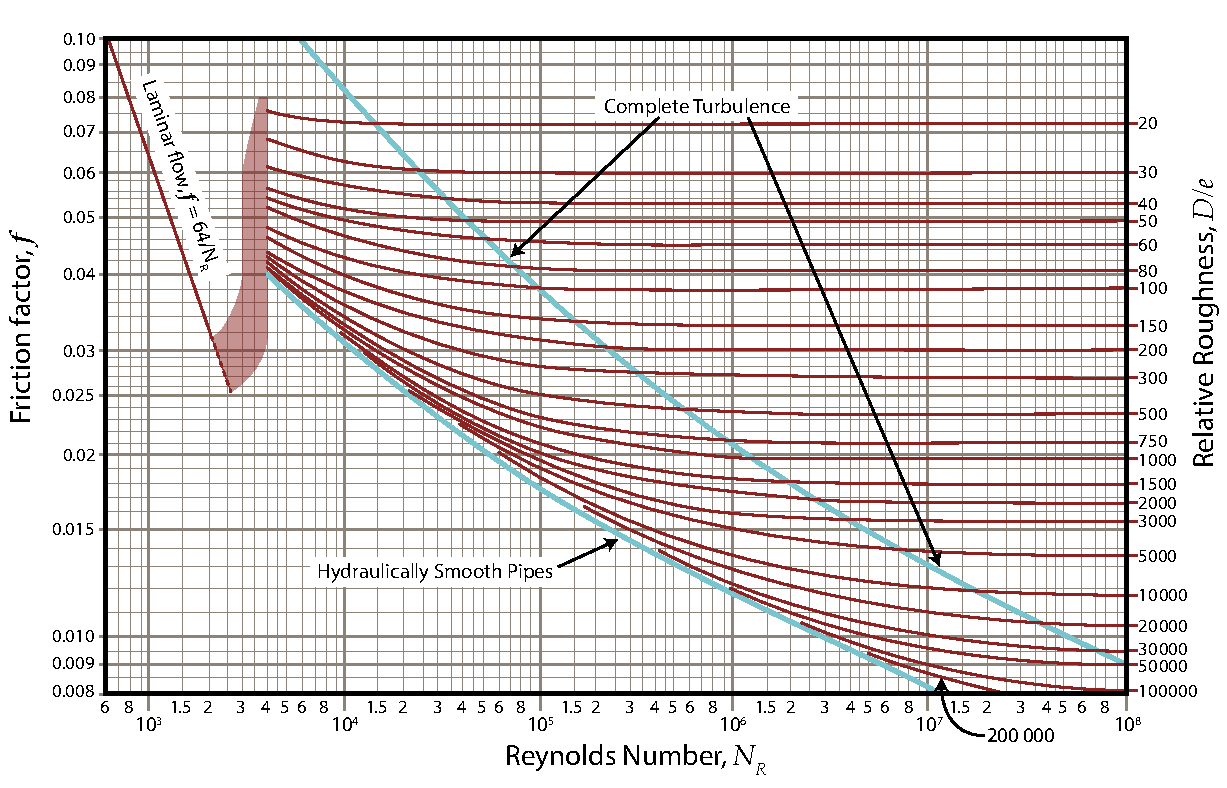
\includegraphics[scale=1.2, angle=90]{../../figs/05FrictionLosses/moody.pdf}
	\end{center}
	
	
	
	
\end{document}
